\documentclass[oneside, 11pt]{article}

\usepackage[T1]{fontenc}
\usepackage[utf8]{inputenc}
\usepackage[dutch]{babel}

\usepackage{fouriernc}
\usepackage[detect-all, load-configurations=binary,
            separate-uncertainty=true, per-mode=symbol,
            retain-explicit-plus, range-phrase={ tot }]{siunitx}

\usepackage{setspace}
\setstretch{1.2}

\setlength{\parskip}{\smallskipamount}
\setlength{\parindent}{0pt}

\usepackage{geometry}
\geometry{marginparwidth=0.5cm, verbose, a4paper, tmargin=3cm, bmargin=3cm, lmargin=2cm, rmargin=2cm}

\usepackage{float}

\usepackage[fleqn]{amsmath}
\numberwithin{equation}{section}
\numberwithin{figure}{section}

\usepackage{graphicx}
\graphicspath{{Figures/}}
\usepackage{subfig}

\usepackage{tikz}
\usetikzlibrary{plotmarks}

\usepackage{fancyhdr}
\pagestyle{fancy}
\fancyhf{}
\rhead{\thepage}
\renewcommand{\footrulewidth}{0pt}
\renewcommand{\headrulewidth}{0pt}

\usepackage{relsize}
\usepackage{xspace}
\usepackage{url}

\newcommand{\figref}[1]{Figuur~\ref{#1}}

\newcommand{\hisparc}{\textsmaller{HiSPARC}\xspace}
\newcommand{\kascade}{\textsmaller{KASCADE}\xspace}
\newcommand{\sapphire}{\textsmaller{SAPPHiRE}\xspace}
\newcommand{\jsparc}{\textsmaller{jSparc}\xspace}
\newcommand{\hdf}{\textsmaller{HDF5}\xspace}
\newcommand{\aires}{\textsmaller{AIRES}\xspace}
\newcommand{\csv}{\textsmaller{CSV}\xspace}
\newcommand{\python}{\textsmaller{PYTHON}\xspace}
\newcommand{\corsika}{\textsmaller{CORSIKA}\xspace}
\newcommand{\labview}{\textsmaller{LabVIEW}\xspace}
\newcommand{\daq}{\textsmaller{DAQ}\xspace}
\newcommand{\adc}{\textsmaller{ADC}\xspace}
\newcommand{\adcs}{\textsmaller{ADC}s\xspace}
\newcommand{\Adcs}{A\textsmaller{DC}s\xspace}
\newcommand{\hi}{\textsc{h i}\xspace}
\newcommand{\hii}{\textsc{h ii}\xspace}
\newcommand{\mip}{\textsmaller{MIP}\xspace}
\newcommand{\hisparcii}{\textsmaller{HiSPARC II}\xspace}
\newcommand{\hisparciii}{\textsmaller{HiSPARC III}\xspace}
\newcommand{\pmt}{\textsmaller{PMT}\xspace}
\newcommand{\pmts}{\textsmaller{PMT}s\xspace}

\DeclareSIUnit{\electronvolt}{\ensuremath{\mathrm{e\!\!\:V}}}

\DeclareSIUnit{\unitsigma}{\ensuremath{\sigma}}
\DeclareSIUnit{\mip}{\textsmaller{MIP}}
\DeclareSIUnit{\adc}{\textsmaller{ADC}}

\DeclareSIUnit{\gauss}{G}
\DeclareSIUnit{\parsec}{pc}
\DeclareSIUnit{\year}{yr}



\begin{document}

\title{\gps calibratie}
\author{A. P. L. S. de Laat}
\date{}

\maketitle

\section{Het \gps systeem}

\gps staat voor Global Positioning System wat vertaald naar wereldwijd
satellietplaatsbepaling systeem. Het is dus een groep satellieten die
radiosignalen uitzenden die het wereldwijd mogelijk maken om te bepalen
waar je bent. Het Amerikaanse project is in 1973 begonnen, het uitvinden
van het systeem wordt toegekend aan Roger L. Easton, Bradford Parkinson
en Ivan A. Getting. Sinds 1994 is het systeem actief. \gps bestaat
momenteel uit 31 satellieten die in banen rond de aarde zijn gebracht.
In \figref{fig:GPSBlockIIIA} is een voorbeeld tekening van zo'n \gps
satelliet. Elke \gps satelliet zit in een baan van ongeveer
\SI{20200}{\kilo\meter} boven de aarde. Zo gaat de satelliet elke 12 uur
om de aarde en zal die elke 24 uur boven de zelfde plek op aarde zijn.
Er zijn ook een aantal tegenhangers van \gps ontwikkeld, namelijk het
Russische GLONASS en het Europeese Galileo\footnote{Dit systeem is nog
niet compleet, maar wordt verwacht binnen een paar jaar operationeel te
zijn.}. Tegenwoordig wordt \gps door bijna iedereen gebruikt, zo zitten
er \gps ontvangers in onder andere telefoons, auto's en ook de \hisparc
electronica.

\begin{figure}
    \centering
    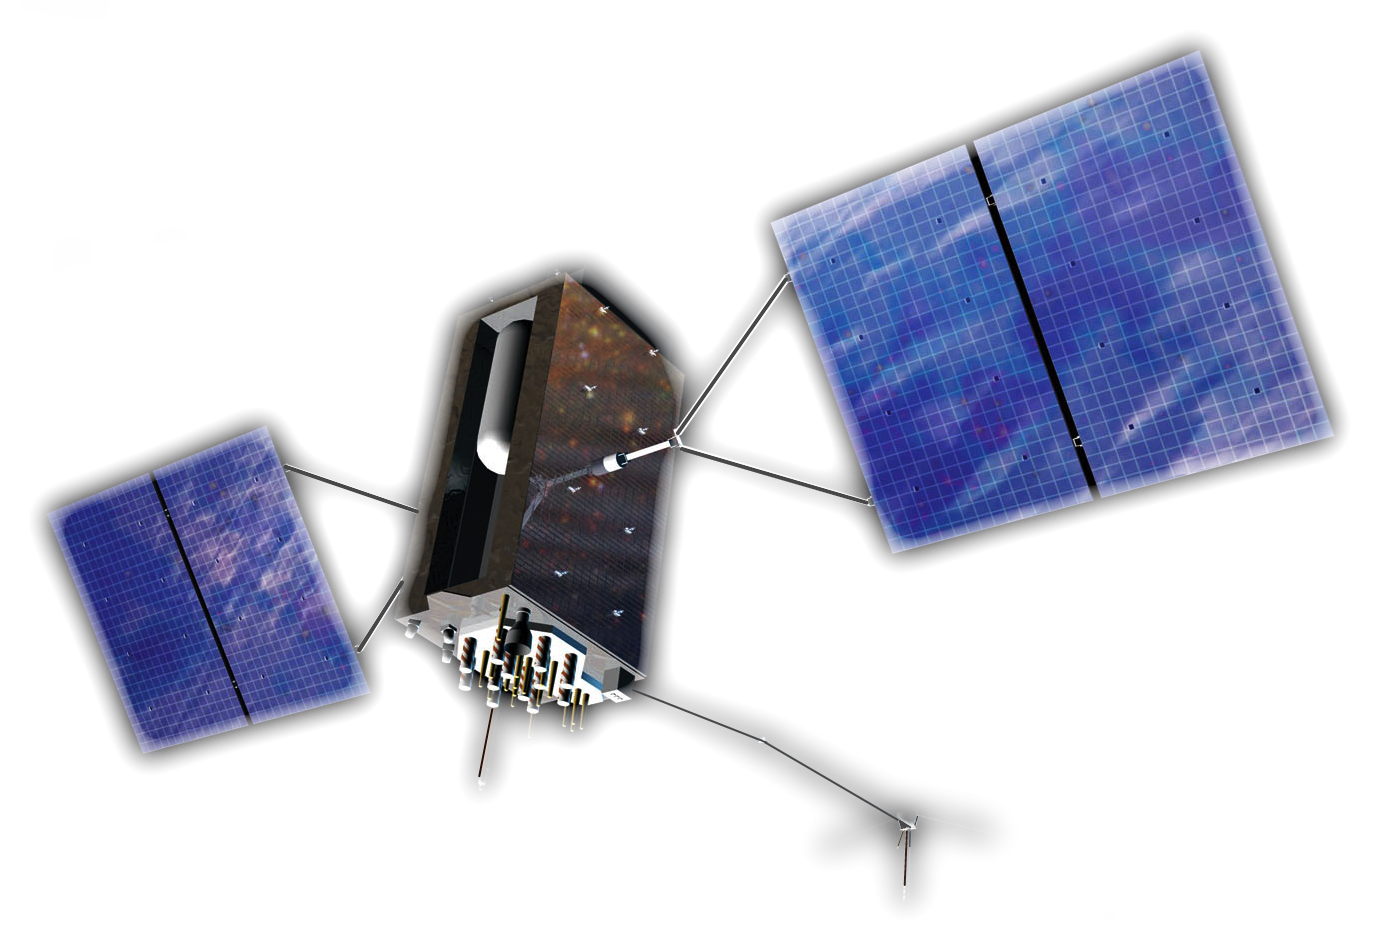
\includegraphics[scale=0.75]{GPS_Block_IIIA}
    \caption{Concept tekening van de nieuwe volgende generatie \gps
    satellieten genaamd \gps Block IIIA. De eerste hiervan wordt in 2014
    gelanceerd. Deze zullen een aantal nieuwe signalen uitzenden en meer
    zendkracht hebben voor hogere accuraatheid voor de gebruikers.}
    \label{fig:GPSBlockIIIA}
\end{figure}

\begin{figure}
    \centering
    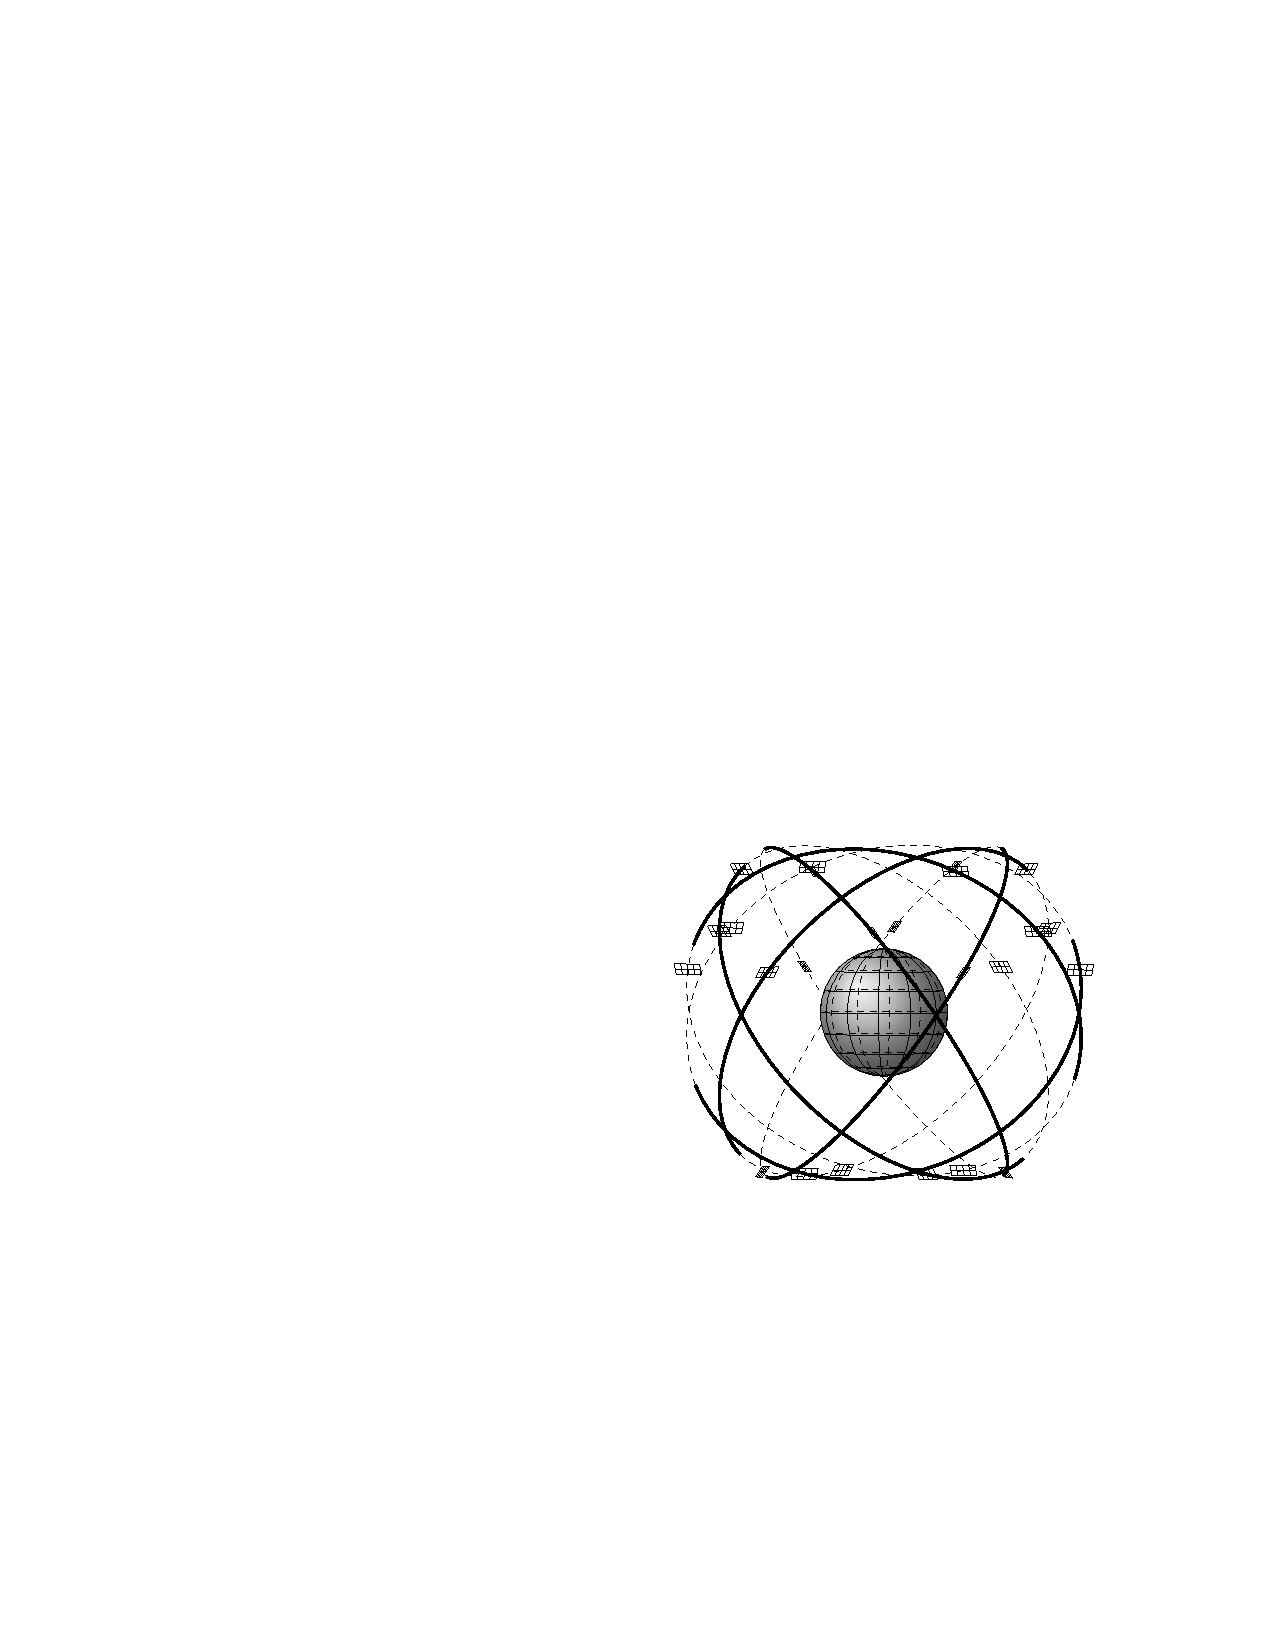
\includegraphics[scale=1]{GPS_satelliet_banen}
    % http://www.ux1.eiu.edu/~kwolcott/3DTikzGraphics.pdf
    \caption{Dit is een schematische weergaven van de banen van de \gps
    satellieten in hun banen rond de aarde.}
    \label{fig:GPS_satelliet_banen}
\end{figure}


\section{Positie bepaling}

Het bepalen van je eigen positie kan met behulp van het weten wat de
afstanden zijn naar 3 andere locaties (niet niet op één lijn liggen),
dit heet trilateratie. Je zal dan namelijk 1 plek vinden die die
afstanden heeft tot de 3 andere punten. De radiosignalen die door de
satellieten uitgezonden worden bevatten informatie over welke satelliet
het zendt, zijn eigen lokatie, de banen van de andere satellieten en de tijd
waarop het bericht verzonden is volgens de satelliet. Door te kijken
naar het tijdverschil tussen het moment waarop een signaal verzonden is
en waarop deze ontvangen wordt kan de afstand tot de satelliet bepaald
worden. Door signalen van meerdere satellieten te combineren kan de
exacte locatie van de ontvanger bepaald worden.

\begin{figure}
    \centering
    \includegraphics[scale=.5]{Trilateratie}
    \caption{Dit is een schematische weergaven van trilateratie.}
    \label{fig:Trilateratie}
\end{figure}


\section{Klokken}
% http://www.staff.science.uu.nl/~gent0113/wettijd/

Vroeger gebruikte men de zon en sterren om een ruwe schatting te maken
van de tijd op de dag. Vanaf de dertiende eeuw werd er in Europa gebruik
gemaakt van mechanische uurwerken, maar deze waren zo onnauwkeurig dat
ze iedere dag aan de hand van de zon moesten worden bijgesteld. In 1656
werd door Christiaan Huygens het slingeruurwerk uitgevonden, deze was
tot op een aantal seconden nauwkeurig over een aantal dagen. Zo'n 10
jaar later ontwierp hij een klok met een spiraalveer die in kleinere
uurwerken gebruikt kon worden, zo kon men ook een nauwkeurigere tijd bij
zich dragen.

Het bijstellen van de openbare klokken werd binnen een stad vaak door
een lokale klokkenmaker gedaan. Dit betekende dat er tussen de meeste
steden wel een tijd verschil was. Naarmate de klokken nauwkeuriger
werden werd het interessanter om betere tijd afspraken te maken binnen
een land. Zo werd in veel Europese landen de middelbare zonnetijd
gebruikt, in Nederland was daar nog weerstand tegen omdat niet elke
gemeente over de financiële middelen beschikte om de nauwkeurigere
klokken aan te schaffen.

Mogelijkheden voor snellere communicatie over langere afstanden
(telegraaf) en sneller reizen (spoorwegen) maakte het halverwege de
negentiende eeuw noodzakelijk om bijna overal in Nederland de middelbare
tijd van Amsterdam aan te houden. Toch was er nog lang onenigheid over
welke tijd precies aangehouden moest worden. Uiteindelijk werd in 1908
een wet aangenomen in Nederland die stelde "De wettelijke tijd in
Nederland is de middelbare zonnetijd van Amsterdam". Later kwamen er
Europese en wereldwijde afspraken over tijdzones, zomer- en wintertijd.

Tegenwoordig wordt tijd bijgehouden door atoomklokken. Deze klokken
hebben een fout van \SI{0.1}{\femto\second} per \SI{1}{\second}. \gps
doet niet mee aan zomer- en wintertijd, en ook niet aan de
schrikkelseconde\footnote{Een extra seconde die af en toe aan de tijd
wordt toegevoegd ter correctie van het verschil tussen de zonnedag en de
\SI{24}{hour} die als dag gezien wordt.}. Dit betekend dat de \gps
precies het aantal seconden sinds 1 January 1970 aangeeft. In het
verleden werkten we met UTC tijd. Maar door de schrikkelseconden kan een
tijdstempel twee keer voorkomen, daarom gebruiken we nu \gps-tijd.


\section{Tijd bepaling}

Als de ontvanger eenmaal zijn eigen positie precies weet, dan kan die
met één satelliet al een precieze tijd bepalen. Dan hoeft namelijk
alleen de afstand tot die satelliet bepaald te worden om zo de reistijd
van het signaal te bepalen. Door dat op te tellen bij de tijd van het
signaal volgt daar de tijd bij de ontvanger uit. Toch worden vaak
meerdere satellieten gebruikt om de tijd nauwkeuriger te krijgen. De
reden hiervoor is dat onder andere de atmosfeer ook effect kan hebben op
het signaal, de signalen van verschillende satellieten gaan door
verschillende stukken van de atmosfeer, door dus gebruik te maken van
meerdere satellieten kunnen deze effecten uitgemiddeld worden.

Elke \gps satelliet heeft een zeer nauwkeurige cesium of rubidium
atoomklok aan boord, deze kan heel nauwkeurig de tijd bijhouden. Hoewel
de \gps satellieten hun tijd goed bij kunnen houden hebben ze wel last
van relativiteit. De klokken in \gps satellieten lijken langzamer te gaan
vanuit ons gezien, doordat ze rond de aarde gaan met zo'n
\SI{14000}{\kilo\meter\per\hour}, maar door de kromming van de ruimte
door de zwaartekracht van de aarde lijkt het juist alsof de klokken in de
\gps satellieten sneller gaan dan op de aarde! Per dag betekend dit dat
de klokken in de satelliet zo'n \SI{38}{\micro\second} op ons voorlopen,
hier wordt natuurlijk voor gecorrigeerd. Dit levert uiteindelijk een
signaal op waarmee we tot \SI{10}{\nano\second} nauwkeurig het begin van
een seconde kunnen aangeven op aarde. De meeste \gps modules geven een
PPS af, een Pulse Per Second, dus elke seconde geven ze aan dat die
seconden begonnen is. In de \hisparc electronica wordt deze PPS gebruikt
om de interne klok te synchroniseren. Tussen de hele seconden wordt de
tijd bij gehouden met een \SI{200}{\mega\hertz} klok. Deze klok wordt op
een slimme manier gebruikt wat uiteindelijk leidt tot een nauwkeurigheid
van $\sigma_t\sim\SI{4.5}{\nano\second}$.
% http://www.phys.lsu.edu/mog/mog9/node9.html


\section{Instellingen}

De \hisparc Master heeft een ingebouwde \gps module. De instellingen van
de \gps worden in het kastje opgeslagen. Het is belangrijk om vóór en af
en toe tijdens gebruik, deze instellingen te controleren. Verder moet de
\gps een zogenoemde "self-survey" uitvoeren om zijn positie vast te
leggen zodat het mogelijk is de \gps als nauwkeurig tijdinstrument te
gebruiken.

Het \gps monitor programma (\dspmon) is te vinden onder onder \hisparc in
het Start Menu. Als in alle tekstvelden een vraagteken staat en de
indicatielampjes op grijs staan heeft het programma de \gps nog niet
gevonden. Rechts onderin het venster kunt u rechts-klikken op "No Com
Port" en de juiste COM poort\footnote{De COM poort identificeerd het
apparaat waarmee de software praat.} selecteren. Ga ze één-voor-één af,
er is er slechts één die zal werken.

Controleert u eerst alle instellingen van de \gps en zorg ervoor dat ze
nauwkeurig overeenkomen met de volgende screenshots (Figuren
\ref{fig:dspmon_receiver}, \ref{fig:dspmon_timing},
\ref{fig:dspmon_survey}, \ref{fig:dspmon_position},
\ref{fig:dspmon_options}). Mocht u een instelling moeten veranderen,
druk dan op de bijbehorende *Set* knop (soms meerdere per scherm).

Vergeet niet na het bepalen van de positie om in de \hisparc \daq de
\daq mode uit en weer aan te zetten om zo de nieuwe positie door te
geven.

\begin{figure}
    \centering
    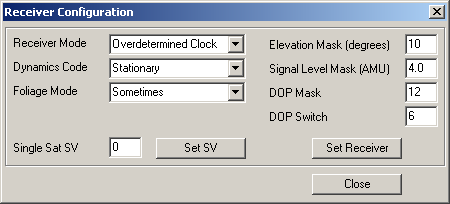
\includegraphics[scale=.75]{dspmon_receiver}
    \caption{In dit venster stelt u de opties in voor de \gps ontvanger. 
    De belangrijkste optie is hier de Receiver Mode.}
    \label{fig:dspmon_receiver}
\end{figure}

\begin{figure}
    \centering
    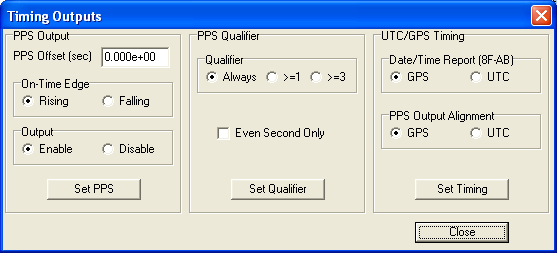
\includegraphics[scale=.75]{dspmon_timing}
    \caption{In dit venster stelt u de tijdsinstellingen in. Het is
    zeer belangrijk om hier goed te controleren dat u \gps meet, en
    geen UTC-tijd.}\footnote{In het verleden hadden we de lengte van de
    self survey ingesteld op één uur, maar het blijkt dat we de
    nauwkeurigheid van een dag nodig hebben.}
    \label{fig:dspmon_timing}
\end{figure}

\begin{figure}
    \centering
    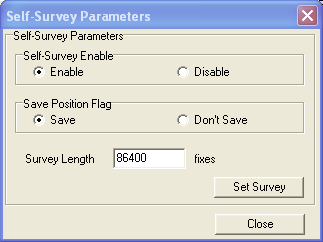
\includegraphics[scale=.75]{dspmon_survey}
    \caption{In dit venster zorgt u er voor dat de *self survey* lang
    genoeg duurt (één dag, dus 86400 seconden).}
    \label{fig:dspmon_survey}
\end{figure}
   
\begin{figure}
    \centering
    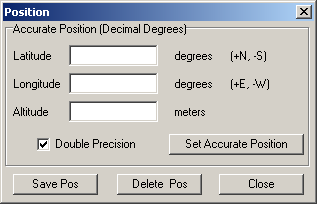
\includegraphics[scale=.75]{dspmon_position}
    \caption{Dit venster kan gebruikt worden om een eerste schatting van
    de positie in te vullen, maar let hier mee op dat deze niet wordt
    vastgezet als definitieve positie. Het is veiliger om deze
    instellingen leeg te houden en de \gps zelf zijn positie te laten
    bepalen.}
    \label{fig:dspmon_position}
\end{figure}

\begin{figure}
    \centering
    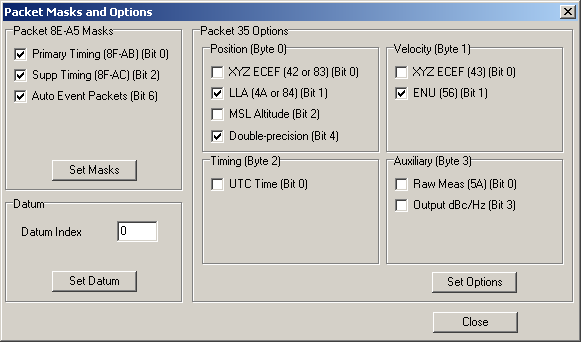
\includegraphics[scale=.75]{dspmon_options}
    \caption{De \gps kent vele opties waarvan een aantal door de \hisparc
    software worden gebruikt. Controleert u deze vinkjes goed.}
    \label{fig:dspmon_options}
\end{figure}



\end{document}
